A migratory typing system adds static types to a
dynamically-typed host language.
At a minimum, the addition requires a static type checker and an extended
syntax to accomodate mixed-typed code.
If the types are intended as claims about the kinds of values that
flow through a program at run-time, then the addition also requires a method
of enforcing types.

Typed Racket~\cite{tf-popl-2008} is one example of a migratory typing system; it adds
a new language, \racketcode{\#lang typed/racket}, to Racket.
The language accepts type-annotated Racket programs,
validates the annotations with a type checker,
and enforces the annotations with higher-order contracts.
For example, \figureref{fig:guess-game} presents a mixed-typed
program consisting of three modules.
The two untyped modules at the top of the figure define a guessing game
and a game player.
The typed module at the bottom gives the player five chances to submit a
correct guess.

Technically, both the guessing game and the player are represented as functions
and the typed driver module assigns a static type to each function.
At compile-time, the type checker validates the contents of the driver module
assuming that the types assigned to the untyped functions are correct.
At run-time, higher-order contracts dynamically enforce the claims in the types.
Thanks to the contracts, these types are kept honest---if a different player
function were to submit a string as a guess, a contract violation would halt
the program.

\begin{figure}[h]
  \begin{minipage}[t]{0.45\columnwidth}
    \begin{lstlisting}
#lang racket
(provide play)

(define (play)
  (define n (random 10))
  (lambda (guess)
    (= guess n)))
    \end{lstlisting}

  \end{minipage}\begin{minipage}[t]{0.45\columnwidth}
    \begin{lstlisting}
#lang racket
(provide stubborn-player)

(define (stubborn-player i)
  4)
    \end{lstlisting}

  \end{minipage}

  \smallskip
  \begin{centering}
    \begin{minipage}{0.6\columnwidth}
      \begin{lstlisting}
#lang typed/racket

(require/typed "guess-game.rkt"
  [play (-> (-> Natural Boolean))])
(require/typed "stubborn-player.rkt"
  [stubborn-player (-> Natural Natural)])

(define check-guess (play))

(for/or ([i : Natural (in-range 5)])
  (check-guess (stubborn-player i)))
      \end{lstlisting}
    \end{minipage}
  \end{centering}

  \caption{A mixed-typed Typed Racket program~\cite{gtnffvf-jfp-2019}}
  \label{fig:guess-game}
\end{figure}

In theory, Typed Racket lets programmers freely mix typed and untyped modules.
The maintainer of a large untyped codebase may add types to any
 one module while leaving the rest untyped.
After the conversion, the new module benefits from static type checking
 and type-driven compiler optimizations; the full mixed-typed codebase can
 be run without further changes.
Running the code may reveal a dynamic mismatch; in particular, an untyped value
 that flows into the newly-typed module may fail to live up to the type annotations.
If so, the program halts and the programmer can fix the types
 and/or the untyped code accordingly.
Adding types thus leads to incremental improvements.

In practice, a programmer's freedom to add types is severly limited by
 the run-time cost of type enforcement.
Adding types to one module adds a contract boundary to its neighbors.
When two modules communicate through a boundary, they may experience three kinds
 of performance overhead.
First, there is the obvious cost of checking every value that crosses the
 boundary.
Second, a higher-order boundary must allocate a new wrappers to constrain the
 future behavior of any values that cross it.
Third, wrapped values suffer from a layer of indirection.
These costs can dramatically increase the running time of a program
 (\figureref{fig:max-overhead}).
Clearly, keeping types honest may impose a huge cost.

\begin{figure}[h]
  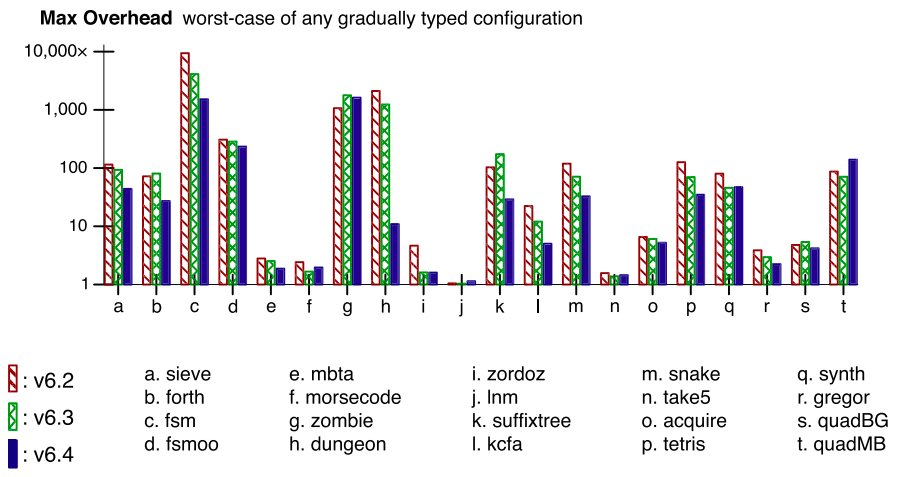
\includegraphics[width=0.8\columnwidth]{src/jfp-2019-max.png}
  \caption{Worst-case overheads across 20 benchmarks and 3 versions of Typed Racket~\cite{gtnffvf-jfp-2019}}
  \label{fig:max-overhead}
\end{figure}
%\footnote{\shorturl{https://}{docs.racket-lang.org/gtp-benchmarks/index.html}}

Other migratory typing systems, however, do not keep types honest in the
 same manner as Typed Racket.
Some add a runtime invariant to reduce the cost of honest types.
Still others choose to selectively enforce types; a value may be obliged to
 satisfy a type is some contexts, but not others.
% TODO explain more
With a few exceptions,\footnote{Like types
 let a programmer toggle between concrete types and erasure.
 Grace enforces user-supplied type annotations with tag checks.
 Pyret enforces user-supplied type annotations with tag checks
  for certain types and a deep traversal for others.}
 the alternatives fall into three broad categories:
 concrete, erasure, and transient.

Stepping back, Typed Racket implements the \emph{natural}\/ type enforcement
 strategy.
A natural semantics carefully guards the boundaries between typed and untyped
 code by wrapping higher-order values in proxies and by eagerly
 checking/traversing other data.
For example, if a natural language expects a list of numbers then it shall
 check every element of an incoming list.
If a natural language expects a function, it shall create a proxy that
 protects future inputs and validates future results.
% On one hand, this strategy lets typed code interact with arbitrary values and
%  ensures that every untyped value completely matches all types associated to it.
% On the other hand, it requires many run-time checks.

A \emph{concrete}\/ migratory typing system comes with two invariants.
First, only statically-typed code can create new values.
Second, every value has an immutable and precise type label.
In a run-time system that enforces these invariants, types can be kept honest
 through label checks.
For example, if a typed function expects a vector of integers and receives
 a value from a dynamically-typed context, it can check whether the value's
 label is a subtype of the expected type.
The value is safe to use if and only if the label is ok.

An \emph{erasure}\/ migratory typing system ignores types at run-time.
Typed code benefits from static type checking, but behaves exactly the same
 as untyped code.
Erased types therefore add zero performance overhead and provide zero feedback
 when statically-typed code receives an input that contradicts the static
 types.
If a typed function receives a bad argument, the application proceeds without
 hesitation and may compute a nonsensical result.

Lastly, a \emph{transient}\/ migratory typing system partially enforces types
 via tag checks.
In typed code, every elimination form and every boundary to untyped code
 is protected with a tag check.
Each tag check matches the top-level shape of a value againt the outermost
 constructor of the expected type; for example, the tag check for a
 list of lists of numbers accepts any list---no matter the contents.
In untyped code, there are no checks.
Transient types are not honest; however, they protect typed code from tag
 errors.

The existence of different approaches indicates a conflict between the theory
 and practice of migratory typing.
Honest types are ideal from a theoretical perspective, but require either
 sophisticated run-time checks or strict limits on the expressiveness of
 untyped code.
Erased types are the polar opposite, as they require no run-time support
 and sacrifice all guarantees.
If researchers can do no better than erasure, then the theory of
 type-sound migratory typing is a dead end.
Transient types suggest a compromise; however, they can mislead a programmer
 and the transient checking strategy imposes overhead on all typed code.
By contrast, natural types are only expensive when typed and untyped code interact.
To illustrate, \figureref{fig:icfp-bars} compares the performance improvement
 in fully-typed Typed Racket code over untyped to the improvement in a
 transient prototype.
Evidently, natural types have better performance in fully-typed programs,
 suggesting the need for a combination.

\begin{figure}[h]
  % TODO log scale, add X for overhead, darker stripes
  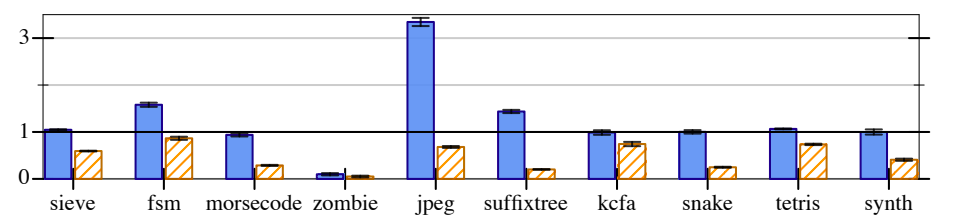
\includegraphics[width=0.8\columnwidth]{src/icfp-bars.png}
  \caption{Speedup factor of Typed Racket vs. untyped (solid bars) and a transient Racket vs. untyped (striped bars)~\cite{gf-icfp-2018}}
  \label{fig:icfp-bars}
\end{figure}


